\documentclass{article}
\usepackage[paperwidth=48in,paperheight=36in,margin=0in]{geometry}
\usepackage[T1]{fontenc}
\usepackage[utf8]{inputenc}
\usepackage{lmodern,amsmath,amssymb,bm,graphicx,xcolor,tikz,booktabs,array}
\usepackage[hidelinks]{hyperref}
% Shared expressions keep the manuscript and poster conventions identical.
\newcommand{\ejab}{\mathit{eJAB}}
\newcommand{\BF}{\mathit{BF}}
\newcommand{\TSBF}{\mathit{TSBF}}
\newcommand{\BFF}{\mathit{BFF}}
\newcommand{\Hnull}{\mathcal H_0}
\newcommand{\Halt}{\mathcal H_1}
\newcommand{\Hplus}{\mathcal H_+}
\newcommand{\Normal}{\mathcal N}
\newcommand{\pto}{\xrightarrow{P}}
\newcommand{\dto}{\xrightarrow{D}}
\newcommand{\TwoSidedFormula}{\sqrt n\exp\!\left\{-\frac12
  \left(1-n^{-1/q}\right)Q_{\chi_q^2}(1-p)\right\}}
\newcommand{\OneSidedFormula}{\frac{\sqrt n\exp\!\left\{
  -\frac12 Q_{\chi_1^2}(1-p)\right\}}{2(1-p_1)}}
\newcommand{\ReconstructedP}{p=2\min\{p_1,1-p_1\}}
\newcommand{\NullPrior}{\theta\mid\Halt\sim\Normal(\theta_0,nv_n)}
\newcommand{\GaussianPosterior}{\theta\mid\boldsymbol y,\Halt
  \ \dot\sim\ \Normal(\widehat\theta,v_n)}
\newcommand{\Rone}{\Pr(p_n\leq\delta\mid\Hnull)\longrightarrow C\delta,
  \quad 0<\delta\leq U_p}
\newcommand{\Rtwo}{D_{q,n}=\sqrt n\,
  \begin{cases}
   -p_n\log p_n,&q=1,\\
   p_n,&q\geq2
  \end{cases}
  \pto0}
\newcommand{\EWDE}{\operatorname{EWDE}}
\newcommand{\NormalizedEWDE}{\operatorname{EWDE}_{\mathrm{norm}}}

\renewcommand{\familydefault}{\sfdefault}
\pagestyle{empty}
\setlength{\parindent}{0pt}
\setlength{\parskip}{0.12in}
\setlength{\emergencystretch}{3em}
\definecolor{navy}{HTML}{173E63}
\definecolor{teal}{HTML}{147D92}
\definecolor{ink}{HTML}{173347}
\definecolor{muted}{HTML}{4A6170}
\definecolor{pale}{HTML}{F0F6F8}
\definecolor{rule}{HTML}{C9DCE3}
\newcommand{\naturalspaces}{\spaceskip=0pt\xspaceskip=0pt}
\newcommand{\bodyfont}{\fontsize{32}{41}\selectfont\naturalspaces
  \setlength{\parskip}{0.13in}}
\newcommand{\leftbodyfont}{\fontsize{30}{37}\selectfont\naturalspaces
  \setlength{\parskip}{0.10in}}
\newcommand{\smallfont}{\fontsize{28}{35}\selectfont\naturalspaces}
\newcommand{\mathfont}{\fontsize{36}{44}\selectfont\naturalspaces}
\newcommand{\subhead}[1]{\par\vspace{0.12in}{\bfseries\color{teal}#1}\par}
\hypersetup{pdftitle={Further developments of generalized Jeffreys's approximate Bayes factor},
pdfauthor={Zhengxiao Wei and coauthors}}

\begin{document}
\null
\begin{tikzpicture}[remember picture,overlay,x=1in,y=-1in]
\begin{scope}[shift={(current page.north west)}]
% Header
\fill[navy] (0,0) rectangle (48,4.12);
\node[anchor=north west,inner sep=0,text=white,text width=29.5in]
at (0.8,0.30) {{\fontsize{64}{70}\selectfont\naturalspaces\bfseries
Further developments of generalized\\
Jeffreys's approximate Bayes factor}};
\node[anchor=north west,inner sep=0,text=white,text width=29.5in]
at (0.82,2.20) {{\fontsize{34}{40}\selectfont\naturalspaces
One-sided eJAB, regularity and Equally Weighted Decision Error Profiles}};
\node[anchor=north west,inner sep=0,text=white,text width=29.5in]
at (0.84,2.94) {{\fontsize{25}{31}\selectfont\naturalspaces
Zhengxiao Wei$^1$, Puneet Velidi$^1$, Evan Strasdin$^1$,
Shreena Nisha Kalaria$^2$, Yimeng Liu$^1$,
C\'eline M.~Laumont$^2$, Brad H.~Nelson$^2$, Farouk S.~Nathoo$^1$}};
\node[anchor=north west,inner sep=0,text=white,text width=29.5in]
at (0.84,3.55) {{\fontsize{21}{26}\selectfont\naturalspaces
$^1$Department of Mathematics and Statistics, University of Victoria
\qquad $^2$Deeley Research Centre, British Columbia Cancer Agency}};

% White department mark and the site's horizontal icon/serif wordmark.
\node[anchor=center,inner sep=0]
at (35.20,2.05) {
\includegraphics[width=9.40in]{figures/uvic_math_stats_white.pdf}};
\node[anchor=west,inner sep=0]
at (41.00,2.05) {
\includegraphics[width=1.60in]{figures/nathoo_group_site_original.png}};
\node[anchor=west,inner sep=0]
at (42.85,2.05) {
\includegraphics[width=3.80in]{figures/nathoo_wordmark_white.pdf}};

% Shared outcome-focused abstract, revised from the user's wording.
\fill[pale] (0.75,4.65) rectangle (20.25,9.70);
\fill[teal] (0.75,4.65) rectangle (20.25,5.50);
\node[anchor=west,inner sep=0,text=white]
at (1.15,5.065) {{\fontsize{39}{45}\selectfont\naturalspaces\bfseries Abstract}};
\node[anchor=north west,inner sep=0,text=ink,text width=18.6in]
at (1.20,5.83) {\smallfontWe further develop and exposit generalized Jeffreys's approximate Bayes
factor (eJAB; Velidi and Wei, 2025). Equally Weighted Decision Error
Profiles compare eJAB with test-statistic Bayes factors (TSBF; Johnson,
2005; Johnson et al., 2023), BIC, and NHST significance rules.
For \(2\times2\) and \(3\times3\) Pearson chi-squared independence tests,
eJAB generally outperforms estimated-\(\omega\) TSBF outside small-sample
or weak-signal regimes; the trend reverses for \(5\times5\) tables.
With true \(\omega\), eJAB generally matches or underperforms TSBF.
BIC differences are small for single-parameter tests; eJAB gains at
weaker effects in multiparameter tests, whereas BIC benefits at stronger
effects. Against \(p<.05\), eJAB gains with larger samples and stronger
signals; weak signals and some small-sample settings favor NHST.
We derive a null-centered one-sided eJAB via the Marsman--Wagenmakers
correction and weaken regularity conditions while retaining consistency.
Three clinical examples illustrate significant findings favoring the null.
};

% Left upper panel
\fill[pale] (0.75,10.10) rectangle (20.25,22.65);
\fill[teal] (0.75,10.10) rectangle (20.25,10.95);
\node[anchor=west,inner sep=0,text=white]
at (1.15,10.515) {{\fontsize{39}{45}\selectfont\naturalspaces\bfseries One-sided eJAB}};
\node[anchor=north west,inner sep=0,text=ink,text width=18.6in]
at (1.20,11.28) {\leftbodyfont
For a scalar parameter, compare \(\Hnull:\theta=\theta_0\)
with \(\Hplus:\theta>\theta_0\).
\subhead{Null-centered encompassing prior}
Let \(v_n=I_n^{-1}(\widehat\theta)\). Use a symmetric prior
centered at \(\theta_0\) and the Gaussian posterior approximation:
\[
 \NullPrior,
 \qquad
 \GaussianPosterior .
\]
With compatible nuisance priors, the Savage--Dickey ratio gives
\[
 \widetilde{\BF}_{01}^{(0)}
 =\frac{\phi(\theta_0;\widehat\theta,v_n)}
        {\phi(\theta_0;\theta_0,nv_n)}
 =\sqrt n\,e^{-W/2},
 \qquad
 W=\frac{(\widehat\theta-\theta_0)^2}{v_n}.
\]
\subhead{Directional mass correction}
The prior mass in the predicted direction is \(1/2\).
For a moderate sample and relatively vague prior,
\[
 \Pr(\theta>\theta_0\mid\boldsymbol y,\Halt)\approx1-p_1,
 \qquad
 \BF_{+1}\approx2(1-p_1).
\]
Reconstruct \(\ReconstructedP\). Substituting
\(W=Q_{\chi_1^2}(1-p)\) gives
{\mathfont
\[
 \boxed{\ejab_{0+}=\OneSidedFormula.}
\]}
\subhead{Finite-sample convention}
The exponent omits \((n-1)/n\); the directional factor
\(1/\{2(1-p_1)\}\) is retained. This is the leading Gaussian
approximation under the null-centered construction.

{\fontsize{26}{33}\selectfont The unrestricted definition retains \(1-n^{-1/q}\)
in its exponent. Its manuscript derivation uses an MLE-centered
prior. The two constructions are distinguished explicitly.}
};

% Left lower panel
\fill[pale] (0.75,23.05) rectangle (20.25,33.90);
\fill[teal] (0.75,23.05) rectangle (20.25,23.90);
\node[anchor=west,inner sep=0,text=white]
at (1.15,23.465) {{\fontsize{39}{45}\selectfont\naturalspaces\bfseries
Regularity and consistency}};
\node[anchor=north west,inner sep=0,text=ink,text width=18.6in]
at (1.20,24.23) {\leftbodyfont\fontsize{29}{36}\selectfont
\setlength{\abovedisplayskip}{6pt}\setlength{\belowdisplayskip}{6pt}
\setlength{\abovedisplayshortskip}{4pt}\setlength{\belowdisplayshortskip}{6pt}
For fixed integer dimension \(q\geq1\), the unrestricted definition is
\[
 \ejab_{01}=\TwoSidedFormula .
\]
\textbf{R1$'$.} Left-tail calibration under \(\Hnull\):
\[
 \Rone .
\]
Here \(0<U_p\leq1\) and \(0<C\leq1/U_p\) are constants.

\textbf{R2 (weakened).} Under a fixed alternative, \(p_n\pto0\) and
\[
 \Rtwo .
\]
Then
\[
 \ejab_{01}\pto\infty\quad(\Hnull),
 \qquad
 \ejab_{01}\pto0\quad(\Halt).
\]
\subhead{Proof sketch}
Under R1$'$, \(W_n=Q_{\chi_q^2}(1-p_n)=O_P(1)\).
Thus \(\log\ejab_{01}=\tfrac12\log n-O_P(1)\pto\infty\).

For \(q\geq2\), \(Q_{\chi_q^2}(1-p)\geq Q_{\chi_2^2}(1-p)=-2\log p\).
Together with the original small-\(p\) bound for \(q=1\), this gives
\[
 0<\ejab_{01}
 \leq n^{1/(2n^{1/q})}D_{q,n}^{1-n^{-1/q}}\pto0 .
\]
These weaker conditions retain consistency under fixed alternatives.
Local sequences \(\theta_n=\theta_0+c/\sqrt n\) may fail R2.
};

% Results occupy the full right column.
\draw[rule,line width=1.4pt] (20.75,4.65) rectangle (47.25,33.90);
\fill[navy] (20.75,4.65) rectangle (47.25,5.50);
\node[anchor=west,inner sep=0,text=white]
at (21.20,5.065) {{\fontsize{39}{45}\selectfont\naturalspaces\bfseries
Equally Weighted Decision Error Profiles}};
\node[anchor=north west,inner sep=0,text=ink,text width=25.5in]
at (21.25,5.83) {\bodyfont
For a specified alternative, equally weighted decision error (EWDE) and its normalized comparison are
\[
 \EWDE_d(\theta,n)=\frac{\alpha_d+\beta_d}{2},
 \qquad
 \NormalizedEWDE(\theta,n)=
 \frac{\EWDE_{\mathrm{comparison}}-\EWDE_{\ejab}}
      {\displaystyle\max_{(\theta,n)\in\mathcal G}
       |\EWDE_{\mathrm{comparison}}-\EWDE_{\ejab}|}.
\]
{\smallfont \textbf{TSBF threshold and optimality.}
For fixed \(\omega>0\) in the chi-squared model, TSBF gives an upper-tail
test that is uniformly most powerful among tests based on \(X^2\)
at its attained size (Neyman--Pearson).
Cutoff \(1\) minimizes prior-predictive error under equal model probabilities
and \(0\)--\(1\) loss. The same cutoff is used for eJAB;
Panel A is a plug-in sensitivity analysis.}
};
\fill[pale] (21.25,9.30) rectangle (46.75,10.95);
\node[anchor=north west,inner sep=0,text=ink,text width=24.9in]
at (21.55,9.48) {\fontsize{30}{38}\selectfont\naturalspaces
\textbf{\color{teal}Panel A: plug-in effect estimate}\qquad
\(\displaystyle
 \widehat\omega=\sqrt{\frac{X^2}{n}},
 \qquad
 \widehat\tau^{\,2}=\frac{n}{q}\widehat\omega^{\,2}=\frac{X^2}{q}.
\)
\par\vspace{0.04in}
{\smallfont \(X^2\): observed chi-squared statistic;
\(n\): sample size; \(q\): degrees of freedom.}
};
\node[anchor=north,inner sep=0]
at (30.50,11.15) {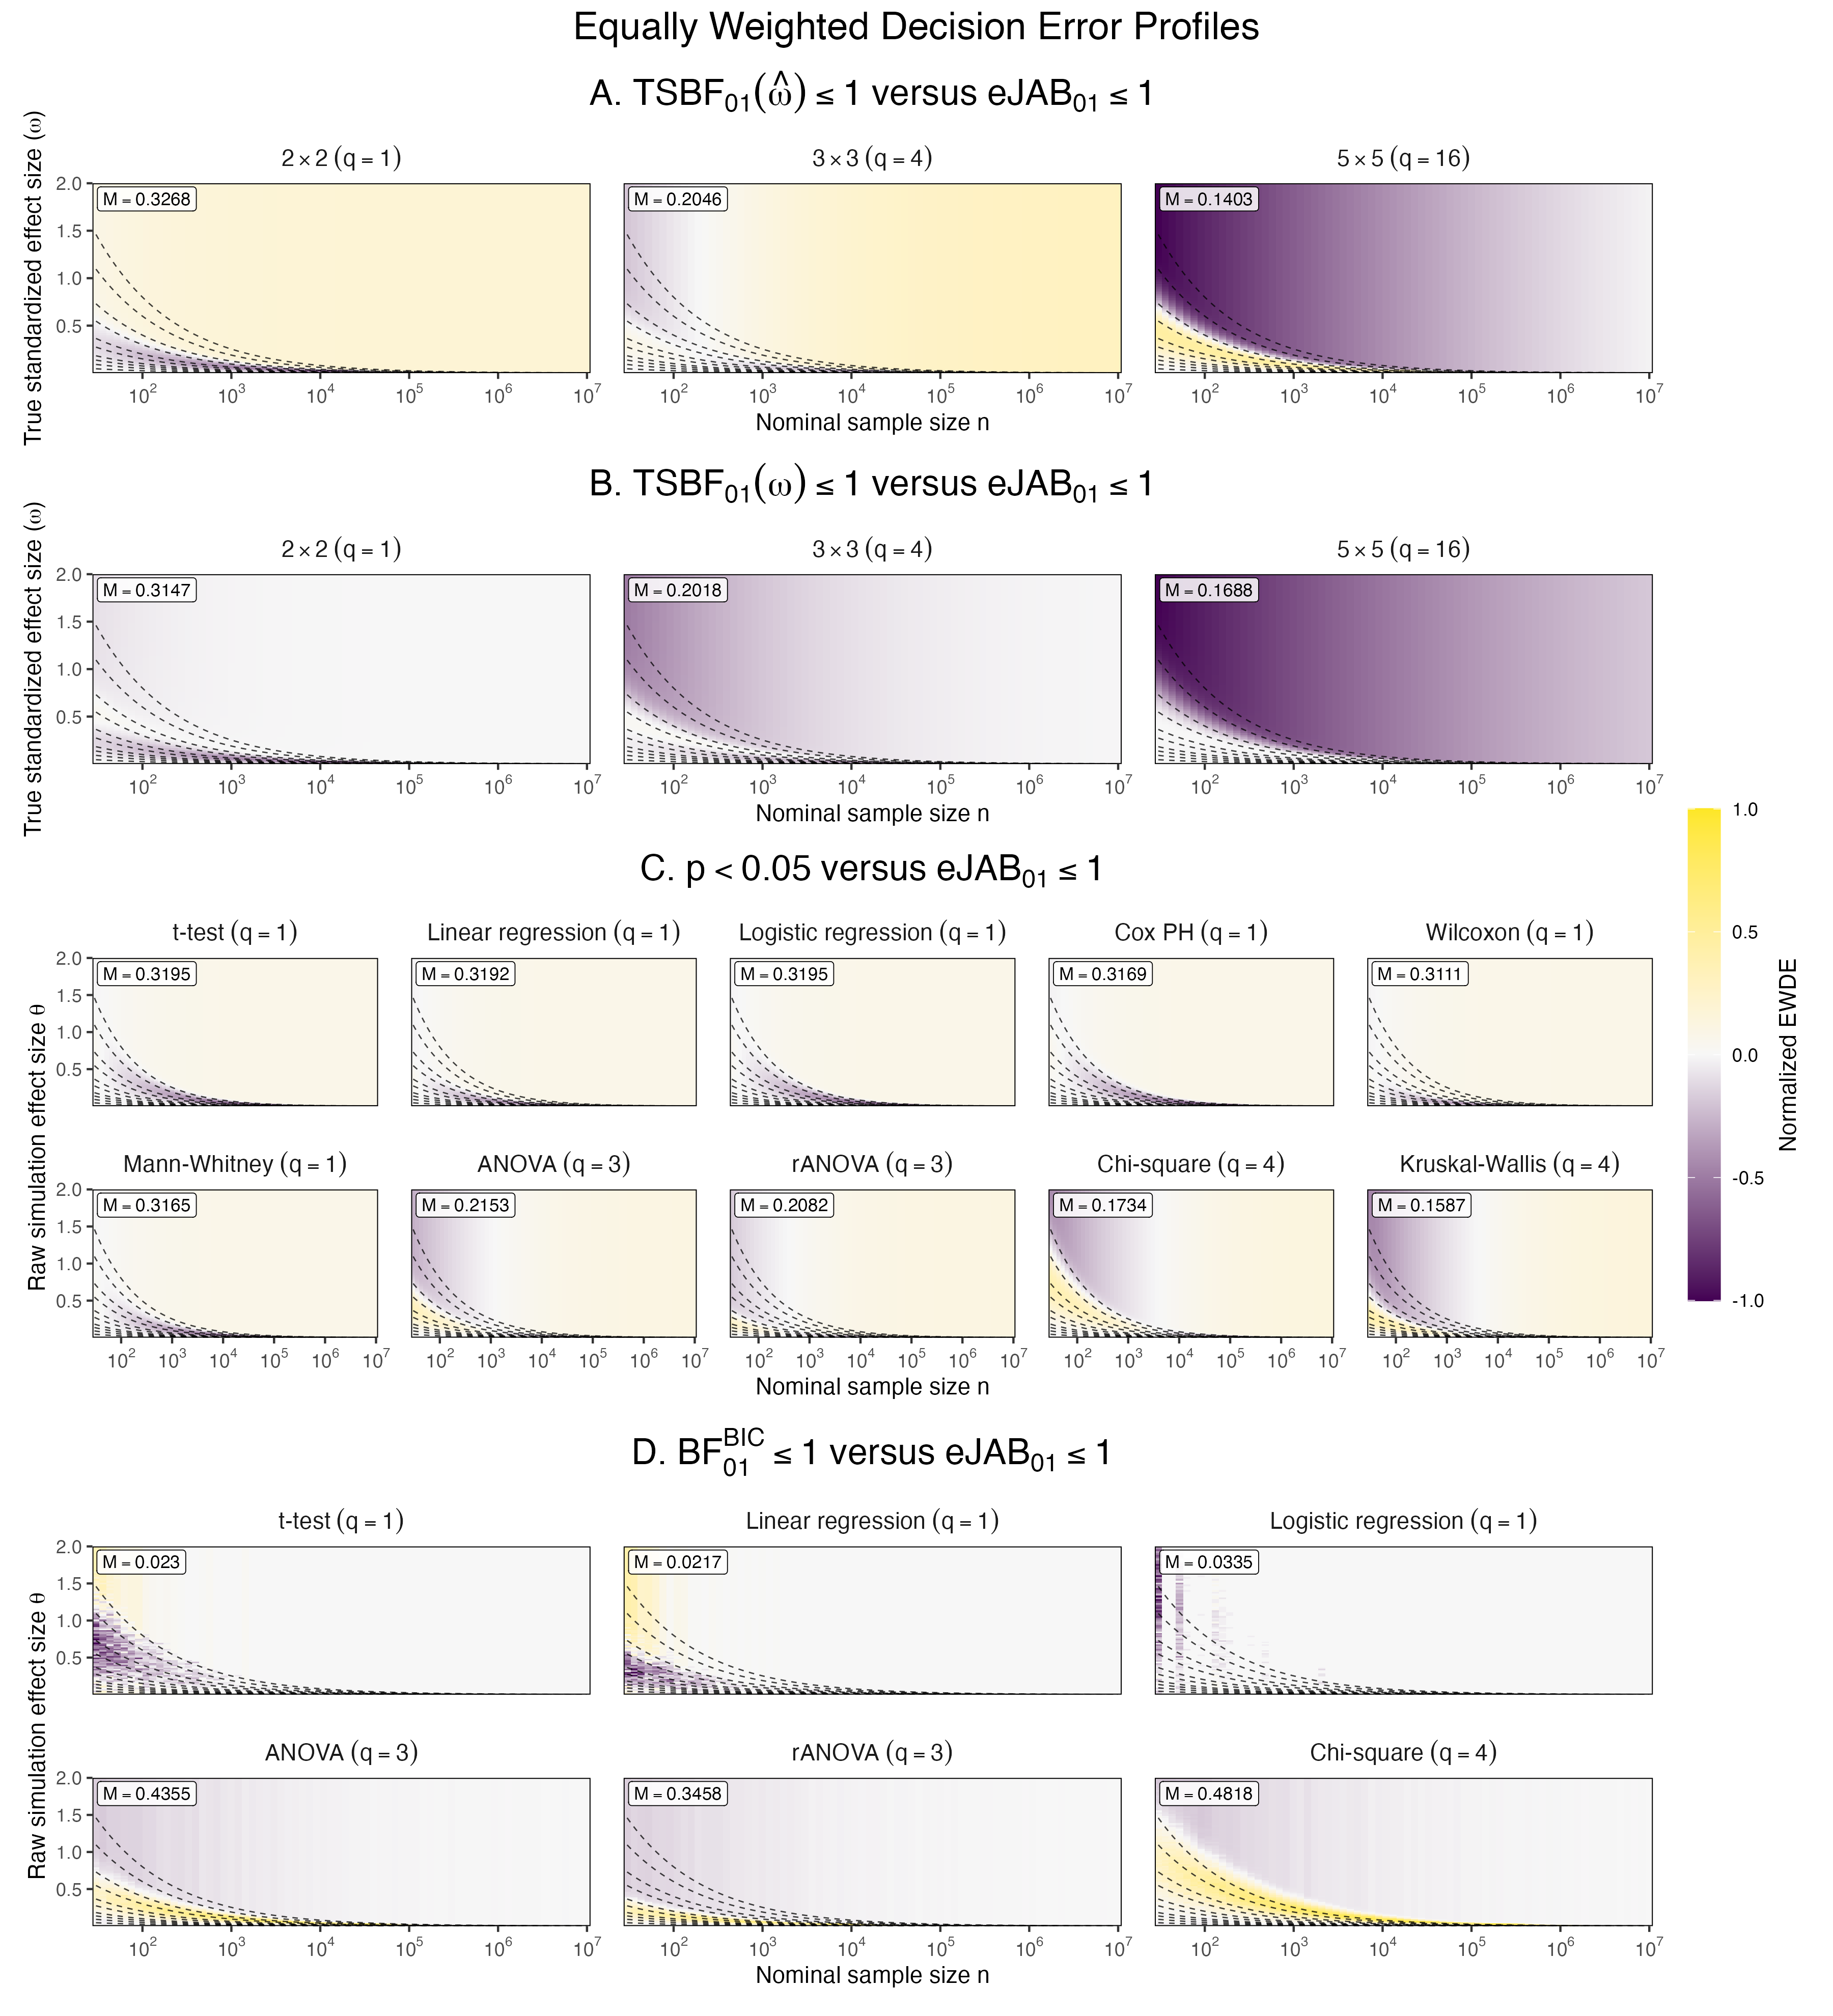
\includegraphics[height=20.40in]{figures/decision_error_profiles.png}};
% Compact application sidebar preserves the profile figure's physical size.
\fill[pale] (40.05,11.40) rectangle (46.75,25.65);
\fill[teal] (40.05,11.40) rectangle (46.75,13.00);
\node[anchor=north west,inner sep=0,text=white,text width=6.05in]
at (40.38,11.58) {{\fontsize{39}{45}\selectfont\naturalspaces\bfseries
Clinical-trial\\contradictions}};
\node[anchor=north west,inner sep=0,text=ink,text width=6.05in]
at (40.38,13.38) {\smallfont
\textbf{Three illustrative examples}
\par\vspace{0.12in}
{\setlength{\tabcolsep}{0pt}\renewcommand{\arraystretch}{1.15}
\begin{tabular}{@{}>{\raggedright\arraybackslash}p{6.05in}@{}}
\toprule
\textbf{Early Phase I}\\
\href{https://clinicaltrials.gov/study/NCT00494806?tab=results}{NCT00494806}\\
First flatus: rocking vs standard care. \mbox{\(t\)-test}.\\
\(n=66,\quad p<.05\)\\
\(\ejab=1.23\)\\
\midrule
\textbf{Phase I}\\
\href{https://clinicaltrials.gov/study/NCT03907683?tab=results}{NCT03907683}\\
Activity after a weekday move-more message. \mbox{\(t\)-test}.\\
\(n=80,\quad p=.037\)\\
\(\ejab=1.04\)\\
\midrule
\textbf{Phase II}\\
\href{https://clinicaltrials.gov/study/NCT00539539?tab=results}{NCT00539539}\\
CPR fraction: feedback on vs off. Linear regression.\\
\(n=1{,}586,\quad p=.016\)\\
\(\ejab=2.19\)\\
\bottomrule
\end{tabular}}
\par\vspace{0.12in}
For \(p<.05\), eJAB uses the bound .05. Contradictions warrant
follow-up; they do not establish Type I errors.
};
\node[anchor=north,inner sep=0,text=ink]
at (43.40,26.12) {{\fontsize{27}{32}\selectfont\naturalspaces\bfseries Paper on arXiv}};
\node[anchor=north,inner sep=0]
at (43.40,26.70) {\href{https://arxiv.org/abs/2510.10358}{
\includegraphics[width=3.0in]{figures/arxiv_qr.png}}};
\node[anchor=north west,inner sep=0,text=ink,text width=18.3in]
at (21.30,31.82) {\smallfont
\textbf{Equally Weighted Decision Error Profiles.}
A--B compare estimated- and true-effect TSBF with eJAB across three
table sizes; C compares \(p<.05\) across ten tests; D compares BIC
across six parametric tests. Colors show normalized EWDE: yellow favors
eJAB; purple favors the comparison. Each panel reports normalization \(M\). Dashed
\(\theta=c/\sqrt n\) curves (\(\theta=\omega\) in A--B) mark constant
standardized signal; normalized EWDE can vary along them.
};
\node[anchor=north,inner sep=0,text=ink]
at (43.40,30.16) {{\fontsize{27}{32}\selectfont\naturalspaces\bfseries Citations}};
\node[anchor=north,inner sep=0]
at (43.40,30.75) {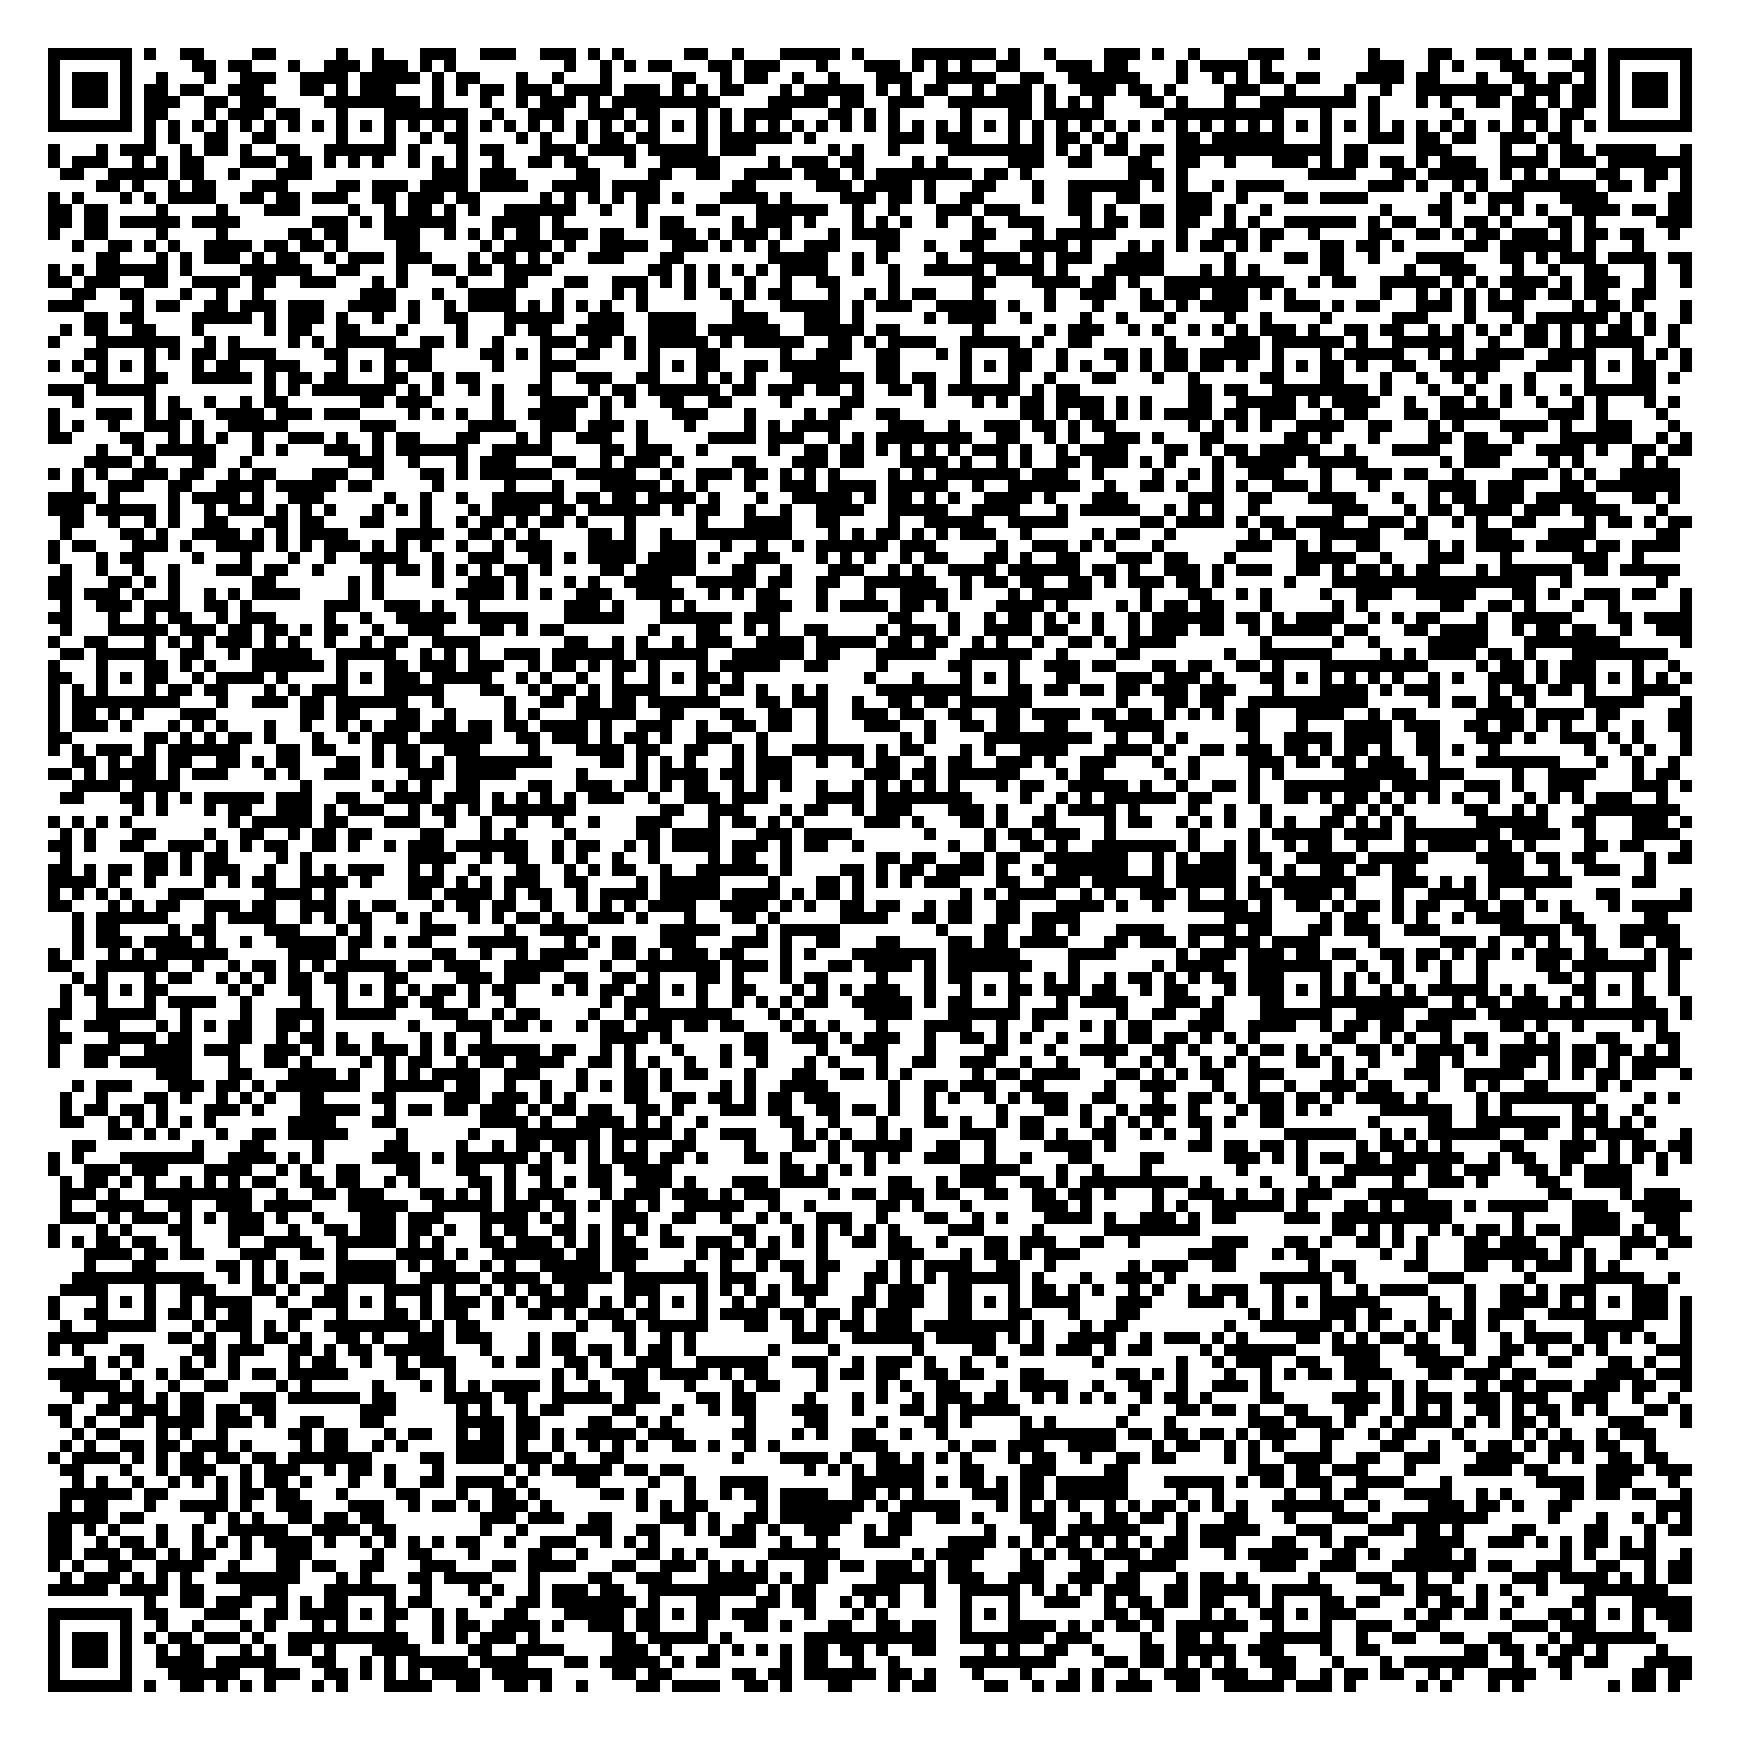
\includegraphics[width=3.0in]{figures/citations_qr.png}};

% References
\node[anchor=north west,inner sep=0,text=muted,text width=40.6in]
at (0.80,34.38) {{\fontsize{18}{23}\selectfont\naturalspaces
\textbf{Selected references}\quad
Velidi and Wei (2025), \emph{Generalized Jeffreys's approximate objective Bayes factor}, arXiv:2510.10358;
Johnson (2005), \emph{Bayes factors based on test statistics}, JRSS B 67, 689--701;\\
Wagenmakers (2022), \emph{Approximate objective Bayes factors from \(p\)-values and sample size};
Marsman \& Wagenmakers (2017), \emph{Educational and Psychological Measurement} 77, 529--539.\\
Mulder, Wagenmakers \& Marsman (2022), \emph{The American Statistician} 76, 102--109;
Johnson, Pramanik \& Shudde (2023), \emph{PNAS} 120, e2217331120;
Fowlie (2021), \emph{Neyman--Pearson lemma for Bayes factors}.}};
\end{scope}
\end{tikzpicture}
\end{document}
